\documentclass[10pt,conference]{IEEEtran}
\IEEEoverridecommandlockouts
% The preceding line is only needed to identify funding in the first footnote. If that is unneeded, please comment it out.
\usepackage{cite}
\usepackage{amsmath,amssymb,amsfonts}
\usepackage{algorithmic}
\usepackage{graphicx}
\usepackage{textcomp}
\usepackage{xcolor}
\usepackage{subfig}
\def\BibTeX{{\rm B\kern-.05em{\sc i\kern-.025em b}\kern-.08em
    T\kern-.1667em\lower.7ex\hbox{E}\kern-.125emX}}
    \def\code#1{\texttt{#1}}
\begin{document}

\title{A Second Look at the Dynamics of the JavaScript Package Ecosystem\\}

\author{\IEEEauthorblockN{Kevin de Haan, Gregory Neagu, Frederic Sauve-Hoover, Abram Hindle}
\IEEEauthorblockA{\textit{Department of Computing Science} \\
\textit{University of Alberta}\\
Edmonton, Canada\\
Email: \{kdehaan,neagu,rsauveho,abram.hindle\}@ualberta.ca}
}

\maketitle

% Footnote should maybe be a full source, or just one link
\begin{abstract}
In recent years, the tools and packages most commonly involved with JavaScript development have evolved rapidly.
Newer packages such as Angular and React have experienced a marked increase in popularity among developers, while frameworks such as jQuery
have begun to phase out.\footnote{\label{adoption}https://insights.stackoverflow.com/survey/2016\#technology-most-popular-technologies, 
https://insights.stackoverflow.com/survey/2017\#technology-\_-frameworks-libraries-and-other-technologies, https://insights.stackoverflow.com/survey/2018\#technology-\_-frameworks-libraries-and-tools}
For this reason we take a second look at a 2016 paper by Wittern, Suter and Rajagopalan \cite{Wittern:2016} to see what aspects of the JavaScript package ecosystem have changed, 
and if previously observed trends have remained constant.
In the original paper the authors use the \emph{node package manager} (\code{npm}) to gain 
insight into the JavaScript ecosystem as a whole, and data from projects publicly hosted on \code{GitHub} to observe an alternative measure of popularity. We adhere to the same methods of analysis, and extend the data to capture
more recent information up to April 1\textsuperscript{st} 2019.
Ultimately, this second look aims to discover if recent years have had any significant effects on ecosystem-wide trends, and provide developers with further insight into how packages are used and evolve.
\end{abstract}

\section{Introduction}
Software ecosystems are environments that form as projects evolve in parallel,
becoming interconnected as contexts and dependencies span companies and communities \cite{LUNGU2010264}. 
Research on these systems has increased rapidly in the recent past \cite{Manikas:2017}, investigating
their characteristics and behaviour as they develop \cite{Manikas:2013}. Understanding how software
ecosystems form and change is important from both a software as well as a business standpoint\cite{Messerschmitt},
and is valuable for informing developers how technologies are used over time \cite{Serebrenik:2015}. 
An understanding of software ecosystems can inform decisions on when to adopt frameworks and how long
to support them, as well as provide insight into how changes to software propagate throughout the community \cite{Wittern:2016}.

This paper is a replication of \emph{A Look at the Dynamics of the JavaScript Package Ecosystem}\cite{Wittern:2016} that performs extensive analysis of 
the \emph{node package manager} (\code{npm}), a popular distributor of JavaScript-based packages. Since the publishing of the original paper, the usage and scale of \code{npm} has only grown. With more than three times as many hosted packages (over 750,000 as of April 1\textsuperscript{st} 2019) 
and over ten times as many weekly package downloads (now over ten billion per week), the raw volume of data and the complexity of package dependency graphs has increased significantly. 
Additionally, the major frameworks used in JavaScript development have undergone a rapid transformation as packages such as Angular and React are adopted\footnotemark[\ref{adoption}].
The core contributions we make are as follows:
\begin{itemize}
  \item We replicate and verify the results found in the original paper for the window of October 1\textsuperscript{st} 2010 to September 1\textsuperscript{st} 2015.
  \item We extend the analysis to the time period of September 2\textsuperscript{nd} 2015 to April 1\textsuperscript{st} 2019, and evaluate whether patterns and trends noted in the original paper are still observable.
  \item We investigate whether the continued evolution of the JavaScript package ecosystem has affected the relationships between various measures of package popularity.
  \item We determine if the ongoing maturation of the JavaScript ecosystem has resulted in tangible changes to version numbering or adoption practices.
\end{itemize}

\section{Related Work}


\section{Data Collection}
% CHECK IF THE NUMBERS ARE RIGHT
The window of data analyzed within this paper is October 1\textsuperscript{st} 2010 (as in the original paper) to April 1\textsuperscript{st} 2019.
We collected from three publicly available data sets. Two of these, the \code{npm} registry and the \code{GitHub} repository platform, are from the same source as in the original paper.
To find repositories relying on \code{npm}, we used the Google BigQuery \code{github\_repos} data set, updated weekly\footnote{https://github.com/fhoffa/analyzing\_github/}.
By using this set we are able to analyze \code{GitHub} data without being constrained to the currently available window provided by the GHTorrent project\cite{Gousi13}.
The final data set encompasses 797,940 packages and \textbf{\#VALUE} applications.

\subsection{Package Metadata}

\textbf{this one is probably mostly for @Fred}

\subsection{Applications using \code{npm} Packages}

\textbf{@Greg I'm gonna need you to put something here}

\section{Ecosystem Evolution}

\begin{figure*}
  % 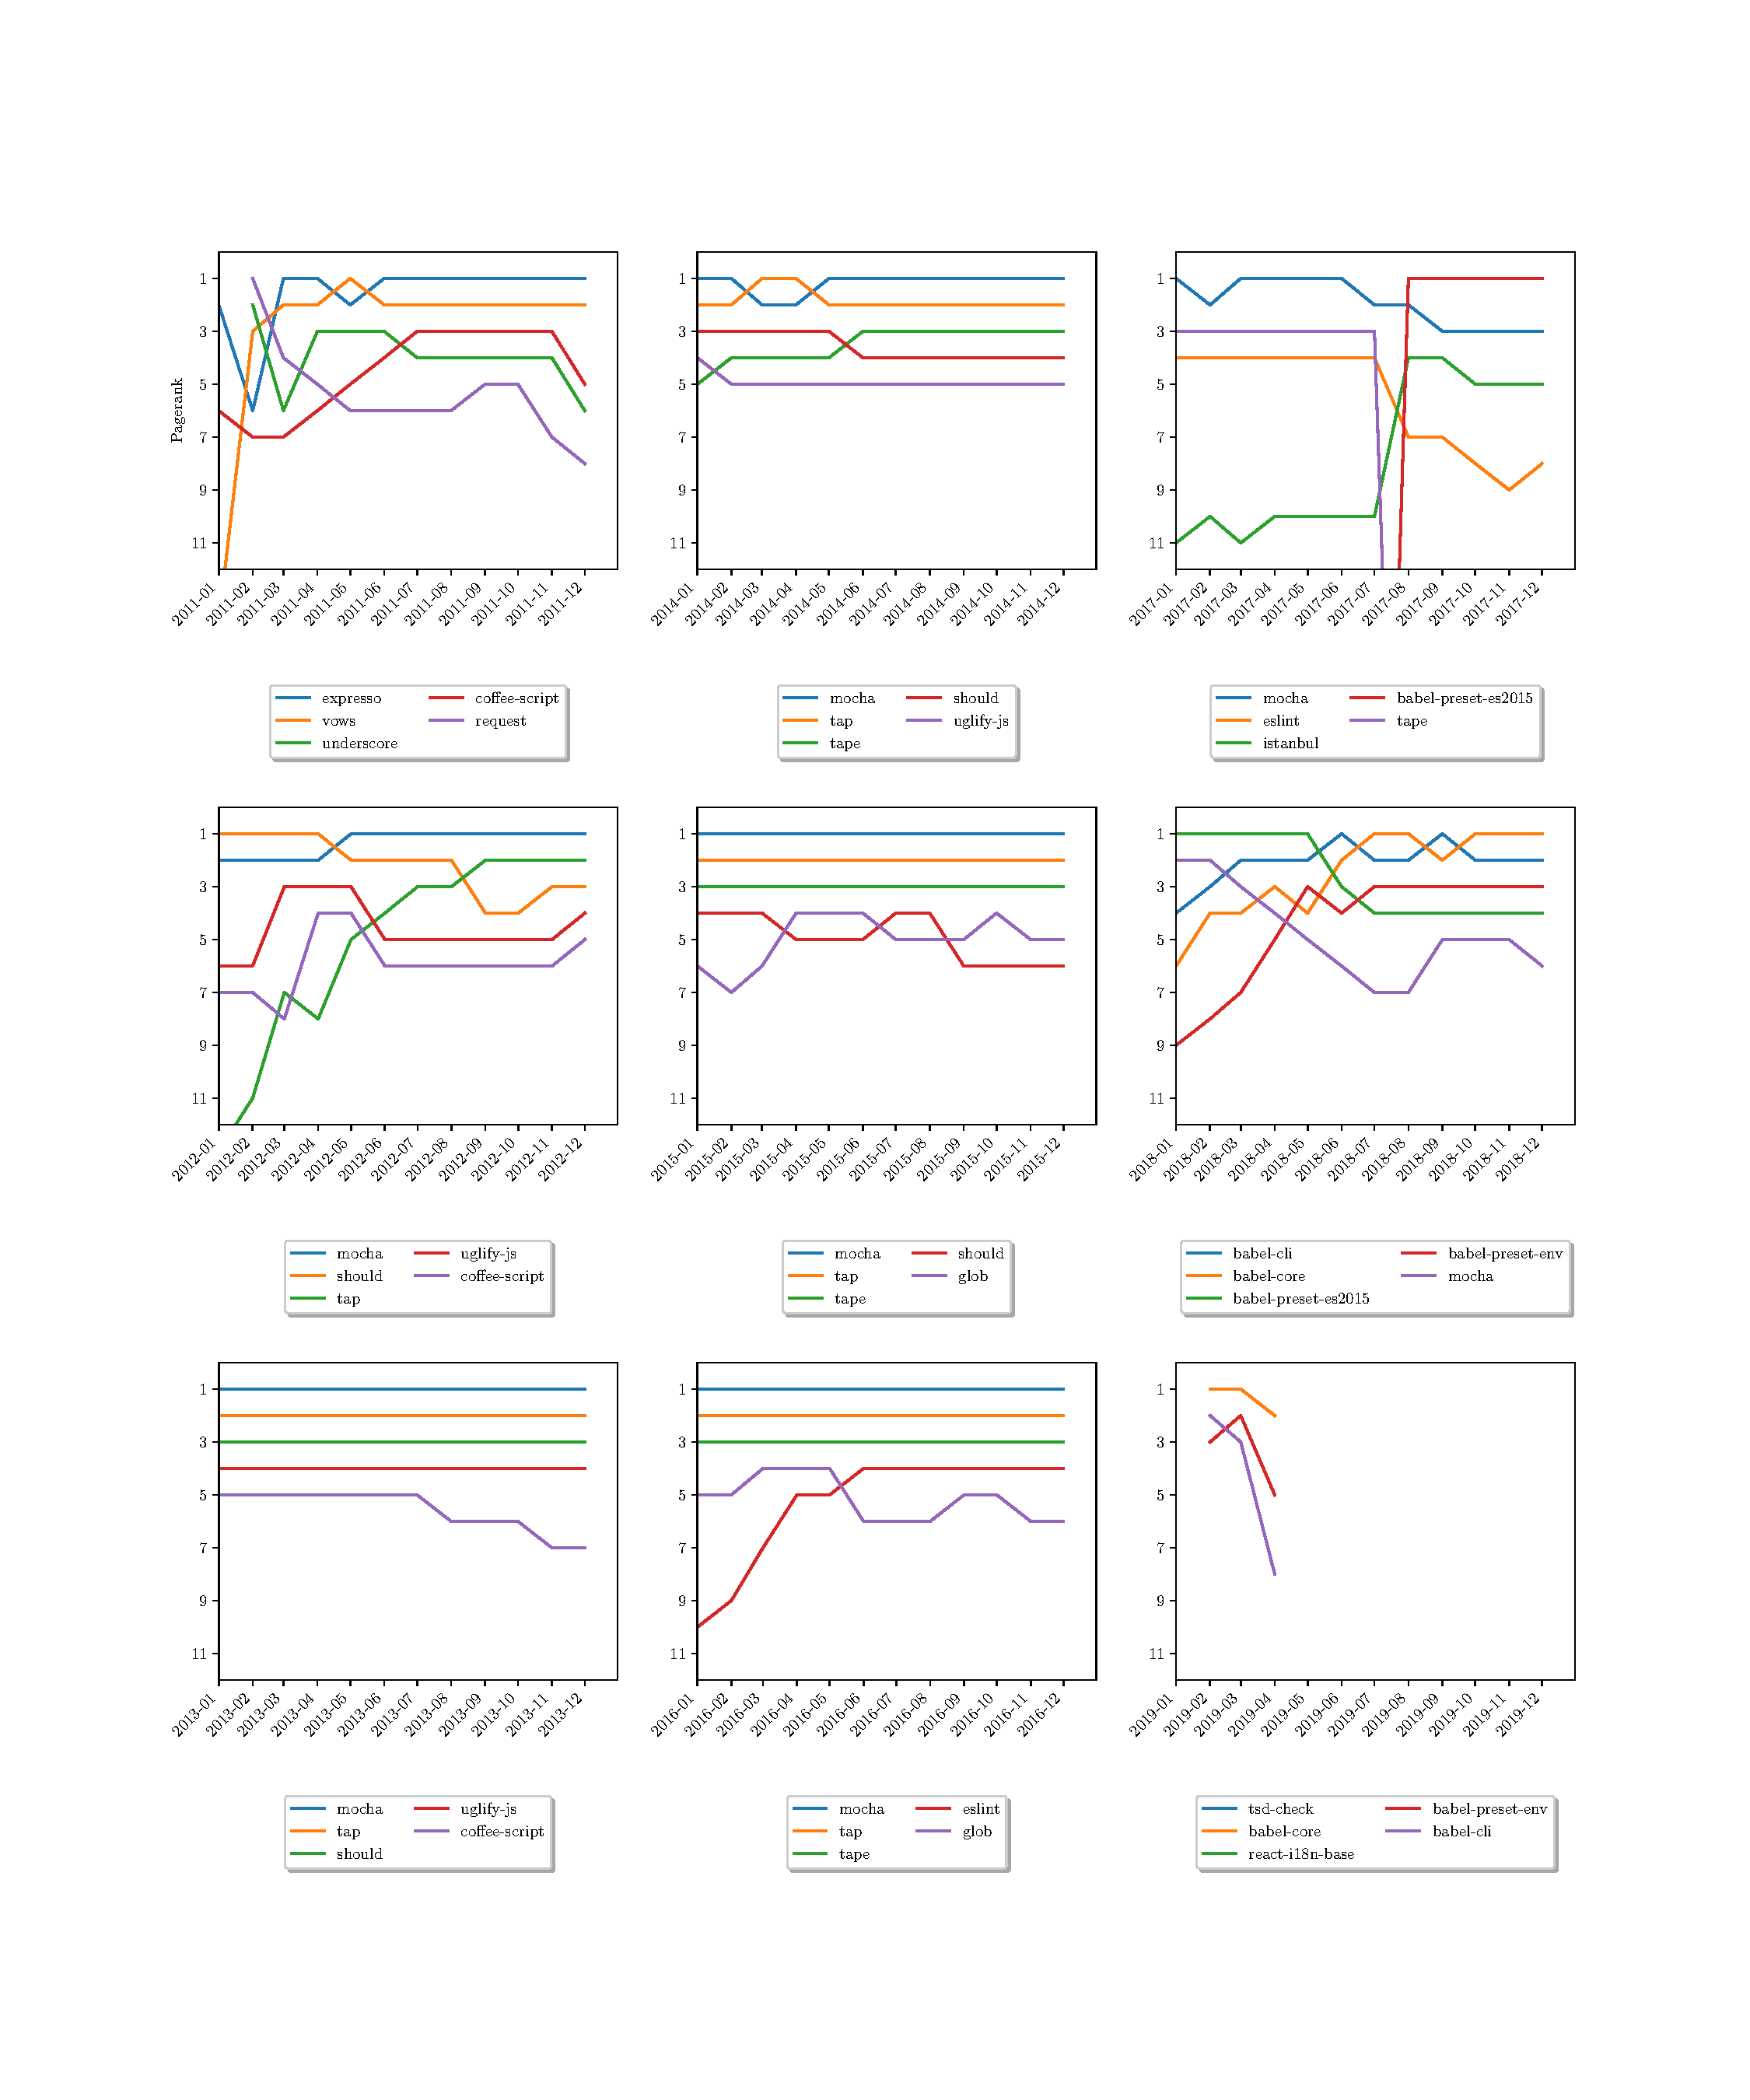
\includegraphics[width=.5\textwidth]{figures/highest_ranked_monthly_100.pdf}

  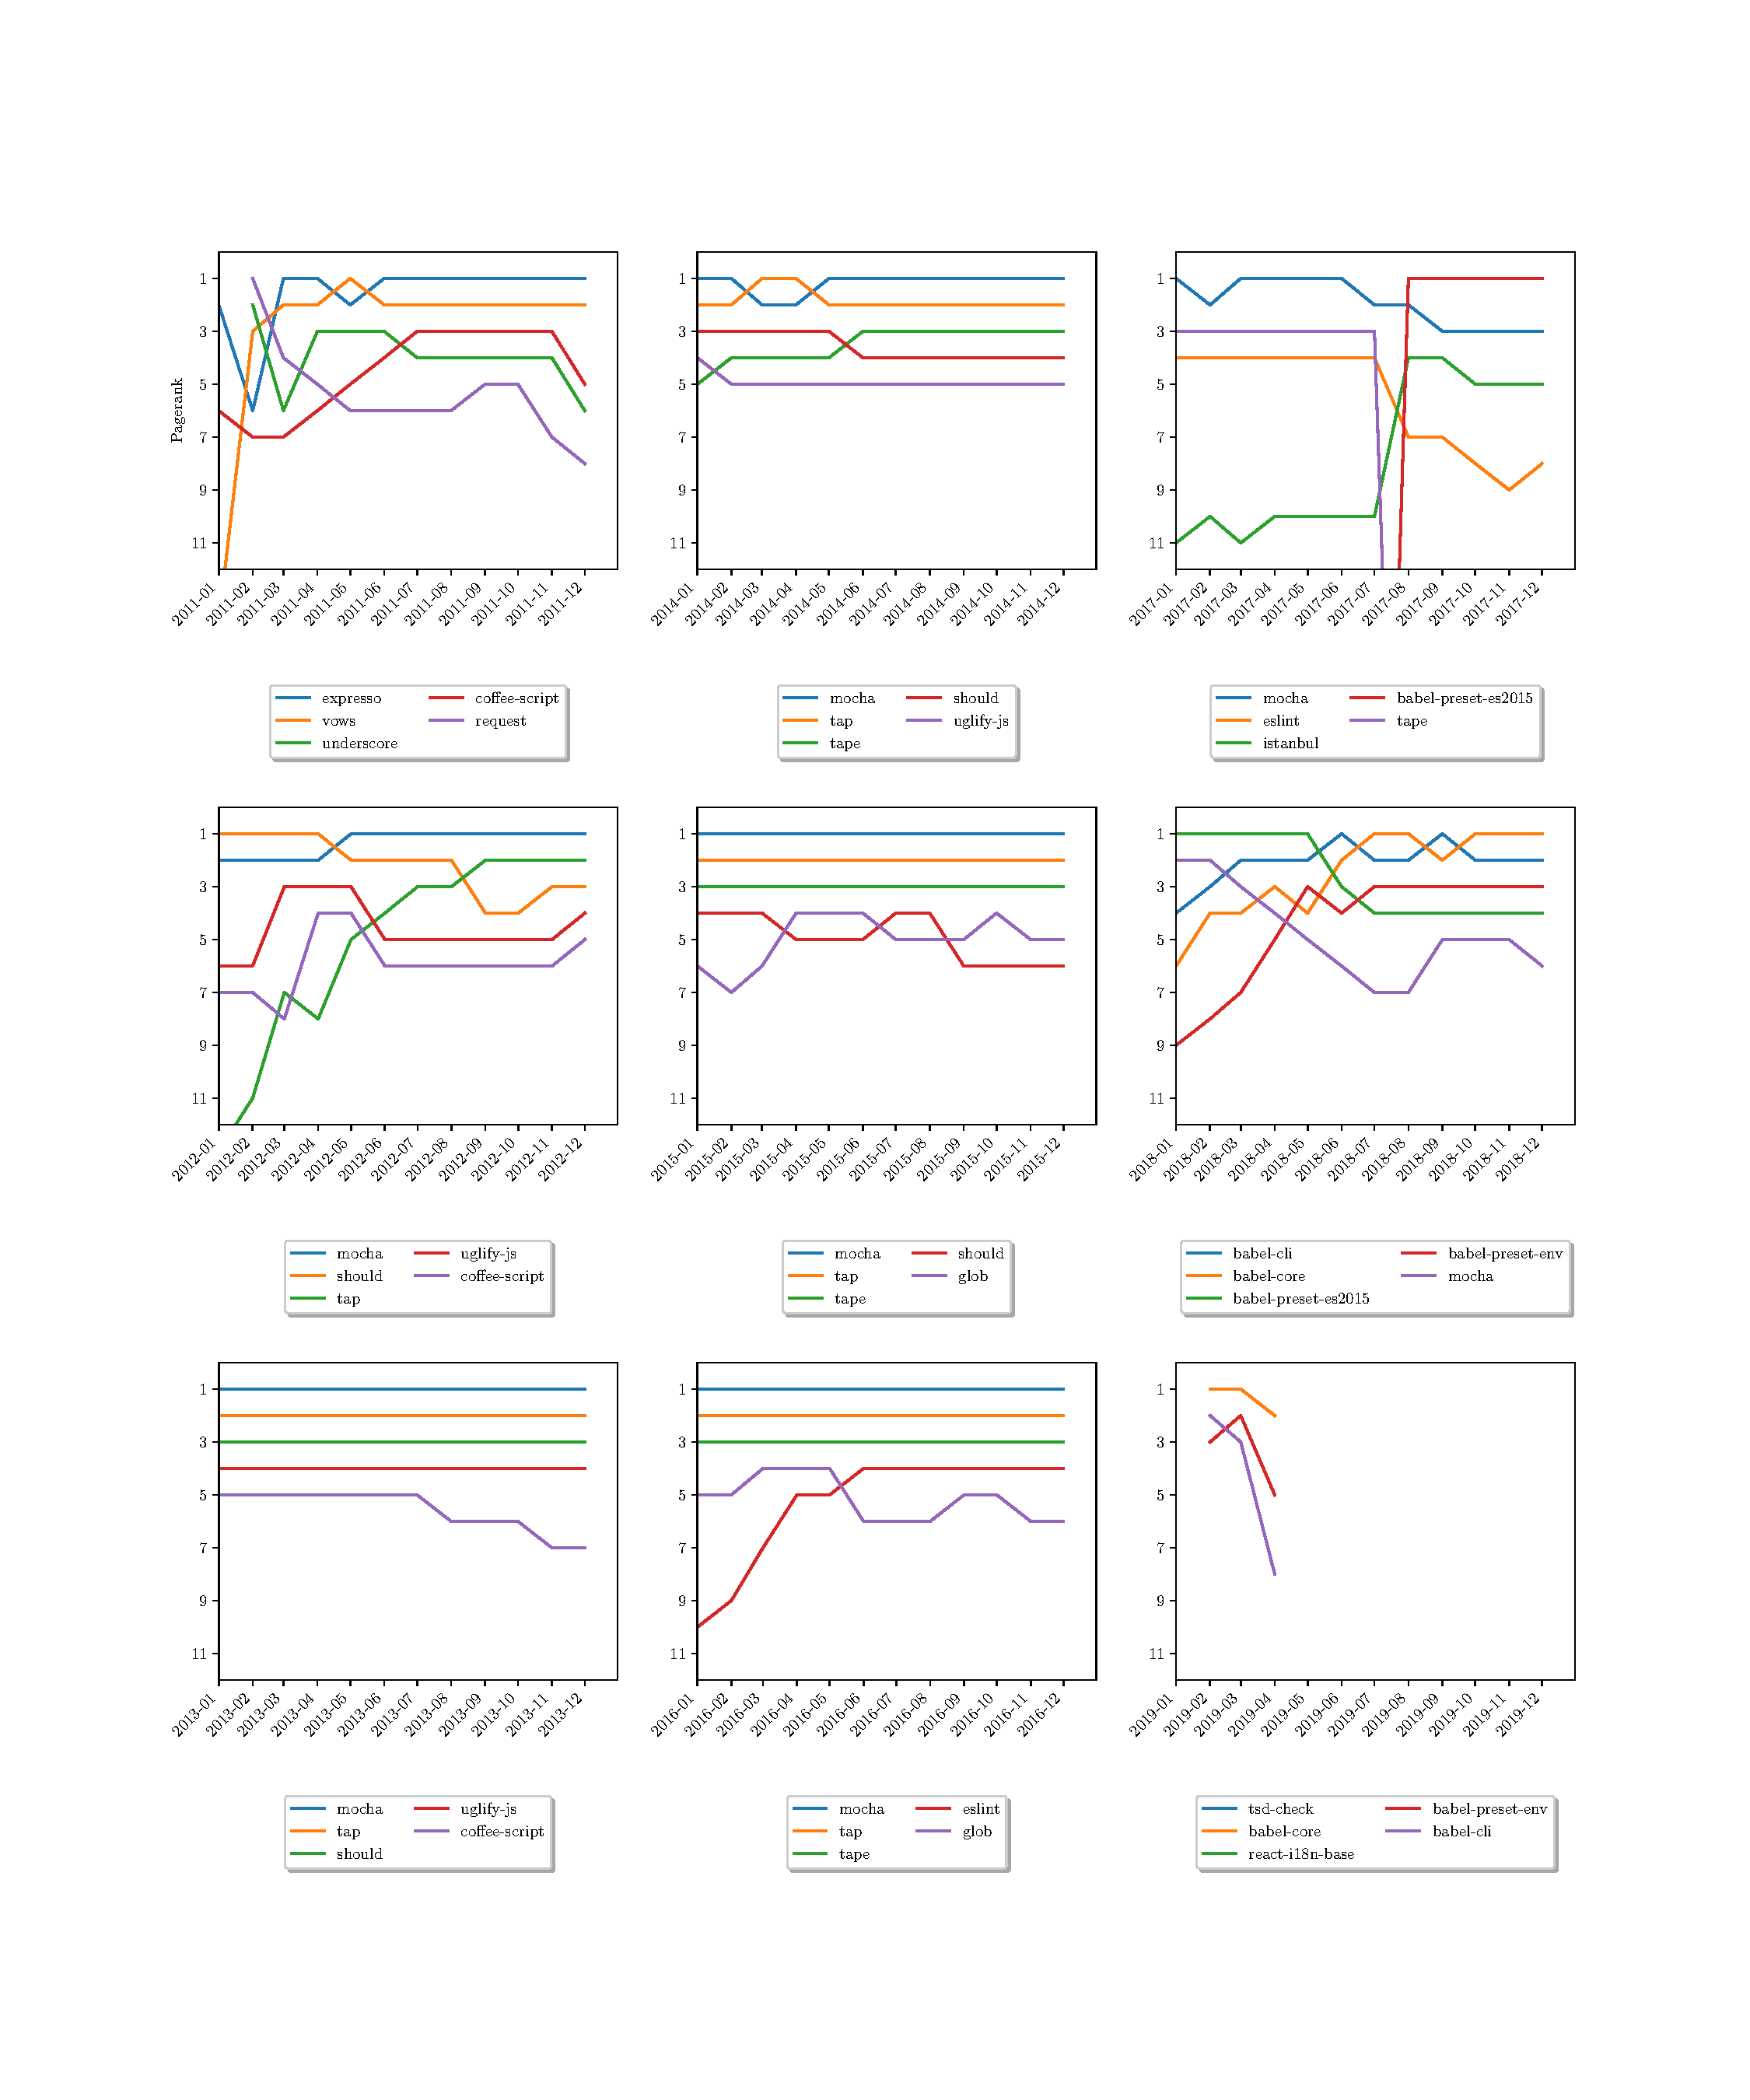
\includegraphics[width=1\textwidth]{figures/highest_ranked_monthly_100.pdf}
  \caption{Neat you can include pdfs}
  \label{ranksByYear}
\end{figure*}

\section{Package Popularity}

\subsection{Relationships between Measures}

\subsection{Distinct Package Types}

\subsection{Popularity Over Time}

\subsubsection{Identifying Top Packages}

\subsubsection{Popular Package Dynamics}

\subsubsection{Comparing Popularities}

\section{Version Numbering and Package Adoption}

\subsection{Attribution of Version Numbers}

\subsection{Adoption by Version Number}

\section{Conclusion}


\begin{thebibliography}{00}

  \bibitem{Blincoe:2015}
  Kelly Blincoe, Francis Harrison, and Daniela Damian.
  \newblock Ecosystems in github and a method for ecosystem identification using
    reference coupling.
  \newblock In {\em Proceedings of the 12th Working Conference on Mining Software
    Repositories}, MSR '15, pages 202--207, Piscataway, NJ, USA, 2015. IEEE
    Press.
  
  \bibitem{Gousi13}
  Georgios Gousios.
  \newblock The ghtorrent dataset and tool suite.
  \newblock In {\em Proceedings of the 10th Working Conference on Mining Software
    Repositories}, MSR '13, pages 233--236, Piscataway, NJ, USA, 2013. IEEE
    Press.
  
  \bibitem{LUNGU2010264}
  Mircea Lungu, Michele Lanza, Tudor Gîrba, and Romain Robbes.
  \newblock The small project observatory: Visualizing software ecosystems.
  \newblock {\em Science of Computer Programming}, 75(4):264 -- 275, 2010.
  \newblock Experimental Software and Toolkits (EST 3): A special issue of the
    Workshop on Academic Software Development Tools and Techniques (WASDeTT
    2008).
  
  \bibitem{Manikas:2013}
  Konstantinos Manikas and Klaus~Marius Hansen.
  \newblock Software ecosystems - a systematic literature review.
  \newblock {\em J. Syst. Softw.}, 86(5):1294--1306, May 2013.
  
  \bibitem{Messerschmitt}
  David Messerschmitt and Clemens Szyperski.
  \newblock {\em Software Ecosystem: Understanding an Indispensable Technology
    and Industry}.
  \newblock 01 2003.
  
  \bibitem{Manikas:2017}
  M.~{Seppänen}, S.~{Hyrynsalmi}, K.~{Manikas}, and A.~{Suominen}.
  \newblock Yet another ecosystem literature review: 10+1 research communities.
  \newblock In {\em 2017 IEEE European Technology and Engineering Management
    Summit (E-TEMS)}, pages 1--8, Oct 2017.
  
  \bibitem{Serebrenik:2015}
  Alexander Serebrenik and Tom Mens.
  \newblock Challenges in software ecosystems research.
  \newblock In {\em Proceedings of the 2015 European Conference on Software
    Architecture Workshops}, ECSAW '15, pages 40:1--40:6, New York, NY, USA,
    2015. ACM.
  
  \bibitem{Wittern:2016}
  Erik Wittern, Philippe Suter, and Shriram Rajagopalan.
  \newblock A look at the dynamics of the javascript package ecosystem.
  \newblock In {\em Proceedings of the 13th International Conference on Mining
    Software Repositories}, MSR '16, pages 351--361, New York, NY, USA, 2016.
    ACM.
  
  \end{thebibliography}
  
\vspace{12pt}

\end{document}
